\documentclass{sigchi}

% Use this section to set the ACM copyright statement (e.g. for
% preprints).  Consult the conference website for the camera-ready
% copyright statement.

% Copyright
\CopyrightYear{2016}
%\setcopyright{acmcopyright}
%\setcopyright{acmlichttps://www.overleaf.com/project/5c9a6fec5ea9cf2e14f83b62ensed}
%\setcopyright{rightsretained}
%\setcopyright{usgov}
%\setcopyright{usgovmixed}
%\setcopyright{cagov}
%\setcopyright{cagovmixed}
% DOI
\doi{http://dx.doi.org/10.475/123_4}
% ISBN
\isbn{123-4567-24-567/08/06}
%Conference
\conferenceinfo{CHI'16,}{May 07--12, 2016, San Jose, CA, USA}
%Price
\acmPrice{\$15.00}

% Use this command to override the default ACM copyright statement
% (e.g. for preprints).  Consult the conference website for the
% camera-ready copyright statement.

%% HOW TO OVERRIDE THE DEFAULT COPYRIGHT STRIP --
%% Please note you need to make sure the copy for your specific
%% license is used here!
% \toappear{
% Permission to make digital or hard copies of all or part of this work
% for personal or classroom use is granted without fee provided that
% copies are not made or distributed for profit or commercial advantage
% and that copies bear this notice and the full citation on the first
% page. Copyrights for components of this work owned by others than ACM
% must be honored. Abstracting with credit is permitted. To copy
% otherwise, or republish, to post on servers or to redistribute to
% lists, requires prior specific permission and/or a fee. Request
% permissions from \href{mailto:Permissions@acm.org}{Permissions@acm.org}. \\
% \emph{CHI '16},  May 07--12, 2016, San Jose, CA, USA \\
% ACM xxx-x-xxxx-xxxx-x/xx/xx\ldots \$15.00 \\
% DOI: \url{http://dx.doi.org/xx.xxxx/xxxxxxx.xxxxxxx}
% }

% Arabic page numbers for submission.  Remove this line to eliminate
% page numbers for the camera ready copy
% \pagenumbering{arabic}

% Load basic packages
\usepackage{balance}       % to better equalize the last page
\usepackage{graphics}      % for EPS, load graphicx instead 
\usepackage[T1]{fontenc}   % for umlauts and other diaeresis
\usepackage{txfonts}
\usepackage{mathptmx}
\usepackage[pdflang={en-US},pdftex]{hyperref}
\usepackage{color}
\usepackage{booktabs}
\usepackage{textcomp}

% Some optional stuff you might like/need.
\usepackage{microtype}        % Improved Tracking and Kerning
% \usepackage[all]{hypcap}    % Fixes bug in hyperref caption linking
\usepackage{ccicons}          % Cite your images correctly!
% \usepackage[utf8]{inputenc} % for a UTF8 editor only

% If you want to use todo notes, marginpars etc. during creation of
% your draft document, you have to enable the "chi_draft" option for
% the document class. To do this, change the very first line to:
% "\documentclass[chi_draft]{sigchi}". You can then place todo notes
% by using the "\todo{...}"  command. Make sure to disable the draft
% option again before submitting your final document.
\usepackage{todonotes}

% Paper metadata (use plain text, for PDF inclusion and later
% re-using, if desired).  Use \emtpyauthor when submitting for review
% so you remain anonymous.
\def\plaintitle{Exploring the Configuration for Multi-user Communication in Virtual Reality}
\def\plainauthor{First Author, Second Author, Third Author,
  Fourth Author, Fifth Author, Sixth Author}
\def\emptyauthor{}
\def\plainkeywords{Authors' choice; of terms; separated; by
  semicolons; include commas, within terms only; required.}
\def\plaingeneralterms{Documentation, Standardization}

% llt: Define a global style for URLs, rather that the default one
\makeatletter
\def\url@leostyle{%
  \@ifundefined{selectfont}{
    \def\UrlFont{\sf}
  }{
    \def\UrlFont{\small\bf\ttfamily}
  }}
\makeatother
\urlstyle{leo}

% To make various LaTeX processors do the right thing with page size.
\def\pprw{8.5in}
\def\pprh{11in}
\special{papersize=\pprw,\pprh}
\setlength{\paperwidth}{\pprw}
\setlength{\paperheight}{\pprh}
\setlength{\pdfpagewidth}{\pprw}
\setlength{\pdfpageheight}{\pprh}

% Make sure hyperref comes last of your loaded packages, to give it a
% fighting chance of not being over-written, since its job is to
% redefine many LaTeX commands.
\definecolor{linkColor}{RGB}{6,125,233}
\hypersetup{%
  pdftitle={\plaintitle},
% Use \plainauthor for final version.
%  pdfauthor={\plainauthor},
  pdfauthor={\emptyauthor},
  pdfkeywords={\plainkeywords},
  pdfdisplaydoctitle=true, % For Accessibility
  bookmarksnumbered,
  pdfstartview={FitH},
  colorlinks,
  citecolor=black,
  filecolor=black,
  linkcolor=black,
  urlcolor=linkColor,
  breaklinks=true,
  hypertexnames=false
}

% create a shortcut to typeset table headings
% \newcommand\tabhead[1]{\small\textbf{#1}}

% End of preamble. Here it comes the document.
\begin{document}

\title{\plaintitle}

\numberofauthors{3}
\author{%
  \alignauthor{Leave Authors Anonymous\\
    \affaddr{for Submission}\\
    \affaddr{City, Country}\\
    \email{e-mail address}}\\
  \alignauthor{Leave Authors Anonymous\\
    \affaddr{for Submission}\\
    \affaddr{City, Country}\\
    \email{e-mail address}}\\
  \alignauthor{Leave Authors Anonymous\\
    \affaddr{for Submission}\\
    \affaddr{City, Country}\\
    \email{e-mail address}}\\
}

\maketitle

\begin{abstract}
  Virtual Reality (VR) enables users to explore scenarios not realizable in the physical world. This allows users to communicate with the help of digital content. We investigate how different configurations of participants and content affect communication in a shared immersive environment. We designed and implemented side-by-side, mirrored face-to-face and eyes-free configurations in our multi-user VR environment and conducted a user study for each configuration, evaluating with respect to ??? within a ??? using the interactive Chalktalk system. We provide experimental results and interview responses.
\end{abstract}

\category{H.5.3.}{Information Interfaces and Presentation}{Computer-supported cooperative work}
\category{H.5.3.}{Information Interfaces and Presentation}{Miscellaneous}
%\category{See  \url{http://acm.org/about/class/1998/} for the full list of ACM  classifiers. This section is required.}{}{}
  %\ccsdesc[500]{Human-centered computing~Mixed / augmented reality}
%\ccsdesc[300]{Human-centered computing~Collaborative interaction}
%H.5.3 Computer-supported cooperative work

\keywords{\plainkeywords}

\section{Introduction}

\section{Related Work}
\subsection{Category 1}
Much work has been done in collaborative applications in VR/MR. T(ether) is a spatially-aware display system for co-located collaborative manipulation and animation of objects ~\cite{lakatos2014t}. Trackable markers on pads and digital gloves allow participants to use gestures to manipulate objects in space. Virtual Replicas for Remote Assistance is a remote collaboration system, allowing a remote expert to guide local users to assemble machine parts by using virtual replicas~\cite{oda2015virtual}.
SpaceTime is a scene editing tool supporting multi-user collaboration in VR, either co-located or remote~\cite{xia2018spacetime}. To support conflict resolution when two users wish to work on the same object simultaneously, SpaceTime creates per-user branches of the object, which can later be merged. 
Rather than enhancing experiences for specific tasks, our system aims to enhance the experience of general communication, which can benefit various kinds of more specific collaborative work.
\subsection{Category 2}
Some previous work contributed to communication in VR/MR too. ClearBoard allows a pair of users to shift easily between interpersonal space and a shared workspace~\cite{ishii1993integration}.
The key metaphor of ClearBoard is ``talking through and drawing on a big transparent glass board.'' No gaze or eye contact information is lost while working on the content. ShareVR enables communication between an HMD user and a non-HMD user~\cite{gugenheimer2017sharevr}. By using floor projection and mobile displays to visualize the virtual world, the non-HMD user is able to interact with the HMD user and become part of the VR experience. The work discusses how people with different devices communicate with each other. MMSpace allows face-to-face social interactions and telepresence in the context of small group remote conferences~\cite{otsuka2016mmspace}. It uses custom-built mechanical displays on which images of remote participants are projected, and which move in response to users' movements. Pairs of participants can maintain eye contact with each other and remain aware of each other's focus. Instead of designing a configuration to fit one specific communication use case, we provide three different configurations for general-purpose communication in VR/MR.

\section{Configuration Design}

\subsection{Side-by-side}

\subsection{Mirrored Face-to-face}

\subsection{Eyes-free}

\section{Implementation}

\subsection{Observation Mode}

\subsection{Interaction}

\subsection{Network}

\subsection{User Study}

\subsection{Participants}

\subsection{Apparatus}

\subsection{Procedure}
\subsubsection{Introduction and Training}
\subsubsection{Experience Three Configurations}
\subsubsection{Questionnaire and Interview}

\subsection{Results}

\subsubsection{The Preference among Configurations}

\subsubsection{Observation Mode}

\subsubsection{Other Findings}

\section{Conclusion}


% Use a numbered list of references at the end of the article, ordered
% alphabetically by first author, and referenced by numbers in
% brackets~\cite{ethics, Klemmer:2002:WSC:503376.503378,
%   Mather:2000:MUT, Zellweger:2001:FAO:504216.504224}. For papers from
% conference proceedings, include the title of the paper and an
% abbreviated name of the conference (e.g., for Interact 2003
% proceedings, use \textit{Proc. Interact 2003}). Do not include the
% location of the conference or the exact date; do include the page
% numbers if available. See the examples of citations at the end of this
% document. Within this template file, use the \texttt{References} style
% for the text of your citation.

% Your references should be published materials accessible to the
% public.  Internal technical reports may be cited only if they are
% easily accessible (i.e., you provide the address for obtaining the
% report within your citation) and may be obtained by any reader for a
% nominal fee.  Proprietary information may not be cited. Private
% communications should be acknowledged in the main text, not referenced
% (e.g., ``[Robertson, personal communication]'').

\begin{table}
  \centering
  \begin{tabular}{l r r r}
    % \toprule
    & & \multicolumn{2}{c}{\small{\textbf{Test Conditions}}} \\
    \cmidrule(r){3-4}
    {\small\textit{Name}}
    & {\small \textit{First}}
      & {\small \textit{Second}}
    & {\small \textit{Final}} \\
    \midrule
    Marsden & 223.0 & 44 & 432,321 \\
    Nass & 22.2 & 16 & 234,333 \\
    Borriello & 22.9 & 11 & 93,123 \\
    Karat & 34.9 & 2200 & 103,322 \\
    % \bottomrule
  \end{tabular}
  \caption{Table captions should be placed below the table. We
    recommend table lines be 1 point, 25\% black. Minimize use of
    table grid lines.}~\label{tab:table1}
\end{table}

\begin{figure*}
  \centering
  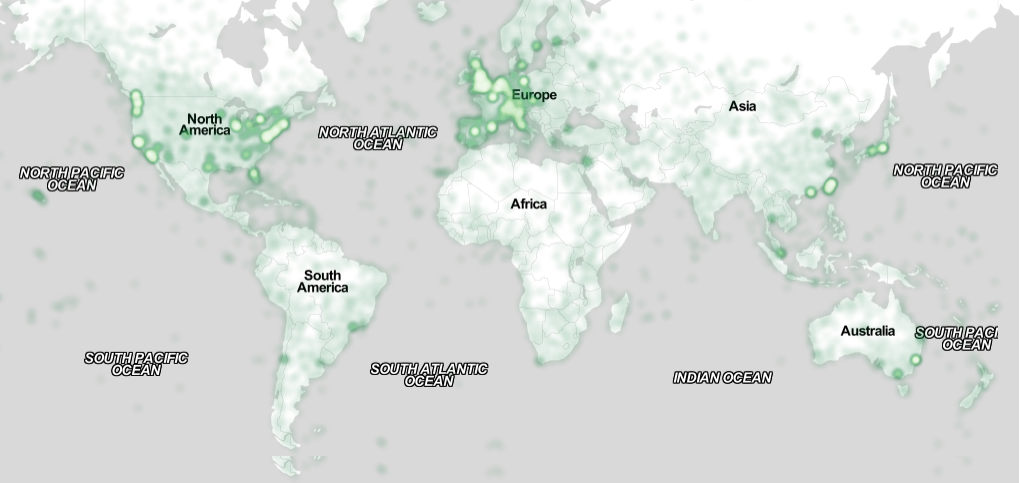
\includegraphics[width=1.75\columnwidth]{figures/map}
  \caption{In this image, the map maximizes use of space. You can make
    figures as wide as you need, up to a maximum of the full width of
    both columns. Note that \LaTeX\ tends to render large figures on a
    dedicated page. Image: \ccbynd~ayman on
    Flickr.}~\label{fig:figure2}
\end{figure*}

\section{Quotations}
Quotations may be italicized when \textit{``placed inline''} (Anab,
23F).

\begin{quote}
Longer quotes, when placed in their own paragraph, need not be
italicized or in quotation marks when indented (Ramon, 39M).  
\end{quote}


\begin{itemize}
\item Write in a straightforward style.
\end{itemize}

\begin{enumerate}
\item Add alternative text to all figures
\end{enumerate}

\section{Acknowledgments}

Sample text: We thank all the volunteers, and all publications support
and staff, who wrote and provided helpful comments on previous
versions of this document. Authors 1, 2, and 3 gratefully acknowledge
the grant from NSF (\#1234--2012--ABC). \textit{This whole paragraph is
  just an example.}

% Balancing columns in a ref list is a bit of a pain because you
% either use a hack like flushend or balance, or manually insert
% a column break.  http://www.tex.ac.uk/cgi-bin/texfaq2html?label=balance
% multicols doesn't work because we're already in two-column mode,
% and flushend isn't awesome, so I choose balance.  See this
% for more info: http://cs.brown.edu/system/software/latex/doc/balance.pdf
%
% Note that in a perfect world balance wants to be in the first
% column of the last page.
%
% If balance doesn't work for you, you can remove that and
% hard-code a column break into the bbl file right before you
% submit:
%
% http://stackoverflow.com/questions/2149854/how-to-manually-equalize-columns-
% in-an-ieee-paper-if-using-bibtex
%
% Or, just remove \balance and give up on balancing the last page.
%
\balance{}

\section{References Format}

% BALANCE COLUMNS
\balance{}

% REFERENCES FORMAT
% References must be the same font size as other body text.
\bibliographystyle{SIGCHI-Reference-Format}
\bibliography{sample}

\end{document}

%%% Local Variables:
%%% mode: latex
%%% TeX-master: t
%%% End:
